\documentclass[conference,letterpaper]{IEEEtran}

\usepackage[english]{babel}


\usepackage[dvips]{graphicx}

\usepackage{graphicx}

\usepackage{longtable}

\graphicspath{{./figs/}}
%%\usepackage[T1]{fontenc}
%%\usepackage[latin2]{inputenc}
%%\usepackage{t1enc}
\usepackage{epsfig}
\begin{document}
\selectlanguage{english}

\title{DroidLab: Mobile Sensing Made Easy, Fast and Cheap}
\author{\IEEEauthorblockN{Bal\'azs Lajtha, Rolland Vida}
  \IEEEauthorblockA{Department of Telecommunications and Media Informatics\\
    Budapest University of Technology and Economics\\
     % Magyar tud\'osok k\"or\'utja 2., Budapest, Hungary, H-1117  \\
    Email: \{lajtha.balazs, vida\}@tmit.bme.hu}}

%\maketitle

% \long\def\symbolfootnotetext[#1]#2{\begingroup  \def\thefootnote{\fnsymbol{footnote}}\footnotetext[#1]{#2}\endgroup}

% \symbolfootnotetext[0]{The second author was supported by the Janos Bolyai
  % Fellowship of the Hungarian Academy of Sciences.}

\maketitle


\begin{abstract}
We are living in a parallelized world. What was thought to be impossible for one can now easily be achieved by many. On one hand, we have the cloud: an army of obeying faceless machines. On the other hand we have the crowd: a colorful collection of volunteers who can be enrolled to perform a specific task. In this paper we present DroidLab, a cloud-backed framework running on Android-based smartphones and supporting the implementation, testing and evaluation of mobile crowd-sourcing applications. Besides describing the architectural elements of the framework, we also present the main challenges of mobile crowd sourcing, and show how DroidLab handles them. DroidLab is still under development, as part of the European research project named EIT ICT Labs FITTING, but many of its elements are already operational. 
\end{abstract}

\begin{IEEEkeywords}
Crowdsensing, Android, Cloud, Gamification
\end{IEEEkeywords}

\section{Introduction}
\label{sec:intro}
"Crowdsourcing is the act of taking a job traditionally performed by a designated agent (usually an employee) and outsourcing it to an undefined, generally large group of people in the form of an open call." This was the initial definition of crowdsourcing when first used in 2006 by Jeff Howe and Mark Robinson \cite{crowdsourcing_definition}. Two main orthogonal problem sets can be solved using crowdsourcing: data gathering and data processing. When a data gathering problem is distributed among members of the crowd we use the term crowdsensing or participatory sensing, while for distributed computational tasks we use the general term crowdsourcing.\\
\indent Another way to categorize crowdsourced applications is whether the contributors profit directly of the gathered or processed information. Wikipedia uses the power of the crowd to provide a service that can directly be used by the contributors. When it comes to crowdsourcing platforms, creating a framework to acquire information is much easier than creating a generic framework that is able to present users with the results. In many cases the beneficiaries of the crowdsourced tasks are different than those providing the data. DroidLab targets these scenarios.\\
\indent Probably the most popular crowdsourced computational problem was SETI@home \cite{Korpela}, a project lasting several years and aimed to search for extraterrestrial intelligence by analyzing radio waves. The problem was divided into a large number of subtasks and distributed among the willing participants. Users could set a SETI screen-saver that downloaded and solved these subtasks when the user was away. SETI's success came from it's innovative design and from the interesting task that it performed. From the point of view of the volunteer, this was a low cost, low gain activity. PCs back than had long startup times and high standby power consumption, so once SETI was installed it didn't generate a visible overhead, and provided the user with an insight of the performed work. Some early gamification elements, like leaderboards, were also implemented.\\
\indent A somewhat different example is the ESP Game \cite{VonAhn2006} classification game, in which two players cooperated to solve a simple puzzle. An image was displayed in both players' browsers. The first player had to find five words that described the image. Then, the second player had to guess those words. This human image processing game allowed to associate more relevant tags to images. The players were motivated to play the game for the game itself, and for added gamification elements.\\
\indent Both examples involved utilization of computational resources owned by the users to perform a highly parallelized task that the users perceived as common good, but they didn't benefit directly from the results of their work. In both cases, users received an input that they processed based on a given algorithm. The tasks were not personalized. SETI@home's tasks were solely performed by a machine, while the ESP Game had to be solved by human users. \\
\indent Participatory sensing on the other hand involves distributed data collection. Sensing can be automated, or can involve the active participation of the user. Before smartphones, sensing was usually done through mostly fixed sensors that were deployed to monitor a given phenomenon at a specific location. They were not able to move, and they had very restricted computational, memory and communication resources, so as to spare their very limited batteries. In case those batteries were depleted, sensors had to be collected, recharged and redeployed, which was a very cumbersome, and sometimes even impossible task. The evolution of smartphones opened the way for many new complex sensing applications. Smartphones have the connectivity that enables real time, high bandwidth communication. The devices can access precise location data, and are equipped with a wide range of sensors from cameras and microphones to accelerometers, gyroscopes and barometers. New mobile operating systems offer many seamless ways for the sensing system to prompt for user input. In addition, smartphones are owned by individuals who recharge them regularly, so energy efficiency becomes less critical.\\
\indent Given these possibilities, a large number of smartphone-based crowdsensing applications emerged recently. However, on one hand, all these applications have several common parts (e.g., communication with the sensor, data collection, data sending, or data processing modules) which are written from scratch by each application developer. In addition, if two or more such applications run on the same phone, they will all consume memory and CPU resources in a redundant and unnecessary way. On the other hand, once the application is written, a large "crowd" of users is needed to test, run and use this application. Gathering such a crowd is however a difficult task, as the users should be motivated in a way to upload and run these specific applications on their personal devices.\\
\indent DroidLab is designed to tackle exactly these issues. First, it provides the research community and the mobile application developers with an easy-to-use skeleton on which they can readily build their own crowdsourcing applications, benefiting from the provided sensing and communication modules. Second, the DroidLab framework will run on a large number of smartphones, enabling application developers to upload their own code on these devices and test it on a large-scale testbed. 
DroidLab is being developed as part of the EIT ICT Labs FITTING European research project, which aims to federate several large scale wired and wireless testbeds, such as PlanetLab, OneLab or SensLab. The goal of the project is to provide a common interface and a transparent access to this large set of heterogeneous resources, enabling researchers to run experiments and test their various protocols and applications. DroidLab adds to FITTING the ability to support mobile nodes and mobility scenarios, a feature that was not addressed by the other, previously mentioned testbeds.\\
\indent DroidLab is a cloud backed mobile platform. The mobile devices participating in DroidLab are called Clients. Clients run the DroidLab framework, which consists of the core and several plugins. The framework is capable of downloading and running crowdsourcing applications, called simply applications. To avoid confusion, users who upload and run their applications over DroidLab will be called Developers. Applications rely on events fired by the plugins and methods offered by the plugins to perform sensing tasks. The framework provides means to the applications for uploading results.\\
\indent The rest of this paper is organized as follows. First, as related work, in section II we present some  promising mobile crowdsourcing applications and frameworks. In section III we  identify the use cases for our DroidLab framework. Then, in section IV we present the architecture of our solution, detailing how our design decisions overcome the common challenges of such platforms. Finally, in section V we conclude the paper and propose some future works.
\section{Related work}
\label{sec:related_work}
We already mentioned two successful examples of crowdsourcing, both targeting desktop platforms. SETI@home was an automated solution while the ESP Game involved user interaction.\\
\indent While it's easy to find proposed applications for participatory sensing, and academic papers discussing the challenges of such applications and their effects on society \cite{Estrin2010}, there is a very limited umber of successfully deployed applications. In 2012 the mobile broadband penetration was  74.8\% in the developed world, but only 19.8\% in the developing world \cite{MobileStats}. While this equals in a larger number of subscribers in the developing regions, most application downloads come from the developed countries \cite{AppDownloads}. Hence, most crowdsourced applications address "first world problems". Here is a short survey of the tackled scenarios, and a brief presentation of some existing crowdsourcing frameworks.
\subsection{Crowd-sensing application scenarios}
Transportation is an area where several crowdsensing applications emerged recently. When using a car, knowing the traffic conditions in advance gives a huge advantage. Waze \cite{Waze} is one of the many traffic aware navigation applications that uses smartphone sensors to identify traffic conditions. Besides traffic, road quality is an important factor too, both for drivers and cyclists. Smartphone acceleration sensors can accurately detect potholes. While no single pothole detection application has emerged, several publications discuss such a framework \cite{Mednis2011}, \cite{Eriksson2008}.\\
\indent When arriving to the destination finding a parking spot will become the main concern. Google launched Open Spot \cite{OpenSpot}, an experimental application that relied on user interaction to detect freed up parking spaces. The application was a failure, and the problem remains unsolved. Finally, public transportation can also benefit of crowdsensed information. HopStop Live \cite{HopStop} is for example an application that provides live transit information gathered by the users.\\
\indent Presence and phone book applications can also benefit of crowdsensing.The user's presence can be detected using sensor information, enabling a framework to communicate detailed information about a contact's state before calling him/her \cite{Miluzzo2008} Phone books can be (partially) shared among users to ease reverse lookup of phone numbers. Mr Number helps its users to avoid unwanted calls by collaboratively maintaining a black list of telemarketers and robocallers \cite{MrNumber}.\\
\indent Weather and environment monitoring is probably the most popular crowdsensing scenario. We participated in the development of the mobile application  Id\"ok\'ep, a Hungarian weather service. Id\"ok\'ep had more than a hundred deployed online weather stations and the mobile application enabled users to share weather photos, perceived weather conditions and analogue measurement results.\\
\indent While smartphones are not equipped with the proper sensors to become a weather station, their near field communication technologies (Bluetooth, WiFi, NFC) enable them to be extended with peripherals capable of measuring air quality, humidity or temperature. In the Common Sense project Bluetooth enabled air pollution sensors were deployed with the mobile application to measure and report air pollutants. Microphones enable smart phones to capture noise level and process noise pollution.\\
\indent Finally, CreekWatch \cite{CreekWatch} is an application that helps to monitor water quality and pollution relying on user reports and photos.\\\indent 
Monitoring network coverage and connection quality can also be done through crowdsensing. The two most important communication channels for smartphones are WiFi networks and cellular networks. WiFi Finder \cite{WiFiFinder} builds and maintains a database of open WiFi networks and their properties. RootMetrics \cite{RootMetrics} on the other hand monitors cellular coverage, as it lets users share their active measurement data to process a coverage map.\\
\indent Healthcare in modern societies is a main concern. Smartphones' sensors can help on many different levels. For individuals it can help to monitor activity, track exercises, with external Bluetooth devices log blood pressure and other metrics. In a family results of the elderly members can trigger alarms at the younger generations. Same can be implemented in a smaller community. On national scale data provides insight of the health level of the people. On a global scale these statistics can help find correlation between lifestyle and health \cite{Jeffrey2006}.\\
\indent A crowdsourced ad-hoc communication network can be useful both on outdoor events where cellular coverage is not designed for many users, and in case of an outage to help first responders contact those without mobile service. Crowd sensing is useful to detect and track parades, estimate number of participants.
\subsection{Crowd-sourcing Frameworks}
Several frameworks have been proposed for different aspects of mobile crowdsourcing, most of them being experimental. mCrowd is a mobile crowdsourcing platform that enables iPhone users to post or tag images or answer questions. mCrowd \cite{Yan} was a prototype application that demonstrated a micro-payment system rewarding the contributors.\\
\indent mClerk \cite{Gupta2012} is a platform that distributes tasks and enables workers to post their responses. mClerk targeted third world users without smartphones. The key challenge of mClerk was to create a communication protocol that enables data transfer over text messages, enabling traditional phone users to receive complex tasks and report results. Both platforms focus on the active contribution of the users.\\
\indent Other frameworks target the communication protocols used in crowdsourcing applications. When information is both gathered and consumed by the same crowd, it is crucial to have a robust, multi-source, multi-destination multicast infrastructure. Fan-Bai et al proposed such a system for vehicular networks. Demirbas et al \cite{Demirbas2010} developed an overlay that uses Twitter to distribute sensor information.\\
\indent Haderer et al \cite{Haderer2013} presented the design of a crowdsensing framework called APISENSE. They identify the main challenges that they face. Their solution, a multi-cloud based SsaS platform focuses on the serving architecture. They promote a multi-tenant approach to increase security, privacy and robustness. APISENSE is composed of a central cloud component and of discrete sensing nodes, each running in the cloud. Sensing tasks are defined using their domain specific language. These definitions are then processed by a Software Production Line that creates the cloud based sensing nodes. Device users are then prompted to join these sensing nodes. APISENSE takes a cloud centric approach, focusing on the gathering, storage and processing of the received data. Aiming to solve the same problem, with DroidLab we take a more client centric approach. Our solution is designed to comply with Android application guidelines. By adjusting DroidLab to the Android eco system, we believe that it will be more appealing and more trustworthy to the users, resulting in higher level of engagement.\\
\indent MEDUSA \cite{Ra} is also an experimental framework that enables the execution of sensing tasks on a swarm of devices connected to a cloud based server. Ryong Ra et al created a scripting language MedScript and a prototype of the runtime. MedScript introduced an abstraction that helps to describe crowdsourcing tasks along with language constructs that map to user involvement, like requesting user input or user actions and rewarding users. MEDUSA also defines a software architecture and provides a reference implementation for cloud-backed crowdsourcing frameworks.\\
\indent As opposed to MEDUSA, DroidLab focuses on automated sensing. We designed our framework to be able to operate in the background, but taking in consideration the user's resources. Our first contribution is a detailed permission and quota management system that gives full control to the users who run the DroidLab framework on their phones.\\
\indent Our second contribution is the plugin-based design that allows the framework to be tailored to the capabilities of the specific device. There exist several thousand different makes of Android devices, dozens of sensors, several different network stack implementations with different feature sets. DroidLab contains different plugins for different sensors. This enables the user to configure his DroidLab installation to match his comfort zone. The plugin architecture is designed to fit Android permission system. The framework's core to require only network access, and every feature requests only privileges crucial to it's operation.\\
\indent Our third contribution is the DroidLab API, a Java API that eases the development of crowdsourcing application with functions to utilize the plugins' functionality, and gives access to sensing related tasks, like scheduling and data collection.\\
\indent In the following section we present the intended use cases of the framework.
\section{Use Cases}
Applications mentioned in the related work sections have several properties in common:\\
- they only work if the contributors reach a critical mass. In location based applications the distribution of the users has to be taken in account too. As Google Play is a global service, an application can reach millions of users, but if these users are scattered around the Globe, some crowd sensing applications will still fail;\\
- they provide services to the users;\\
- provided services can be consumed on the same mobile device, through a specific application;\\
\indent For such an application to succeed, the provided service has to be in balance with the required contribution, and the application has to be advertised and distributed rapidly. These requirements result in well-polished, feature rich applications that emphasize the provided services, and have high marketing costs. If an application doesn't reach enough users or active user contribution is required which is too costly (see Google's Open Spot), the service dies out. This is a high cost, high risk business.\\
\indent A crowdsensing platform on the other hand takes quite a different approach. It doesn't provide value to the user, at least not as directly as a specific application can. The user base doesn't have to grow exponentially to sustain the provided services. DroidLab will host different kinds of applications, in different stages of growth.\\
\indent DroidLab is designed to be used in several ways, with different goals in mind. DroidLab can act as a bootstrapping device for a mobile crowdsensing application. Until the critical user mass is reached, DroidLab nodes can provide the missing information for the crowdsensing service to operate correctly.\\
\indent If a given service requires mobile sensor data, but doesn't offer content to the mobile users, it is especially hard to motivate users to download yet another application that will run in the background and consume resources, without providing any value to the device owner. If a device runs DroidLab, such applications can be deployed seamlessly, without distracting the user. There is no need thus to convince a large group of users to download and run each specific application, they have to be convinced just once, to install the DroidLab framework, and for the same entry cost of a single mobile sensor application, the user will be able to participate in different sensor networks over a long period of time. \\
\indent Finally, DroidLab's initial purpose was to be a research platform, a large-scale mobile test network similar to PlanetLab and SensLab, over which researchers can test their developed algorithms and protocols. This is because it is especially difficult to deploy large-scale applications for research purposes, as they usually don't provide any value to the user, operate only for short periods of times, and usually target specific user groups. DroidLab can be regarded thus as a large-scale testing infrastructure for mobile applications. \\
%\indent The majority of the currently sold phones are smartphones; regardless of their gender, age, and technical knowledge, users are persuaded to buy smartphones, resulting in the wide penetration of these devices. We designed DroidLab so as to not require any maintenance. After the framework is set up on the device and configured properly according to the users' privacy requirements and available resources, it operates in a self-sustained manner, no user interaction being needed. This enables the deployment of DroidLab on devices that are owned by users who are not familiar with modern technology, wideningthe pool of reachable users. With proper marketing and communication, every smart phone user can be targeted. However, the main target group of the DroidLab framework are students and young adults , owning smartphones with mobile broadband access, who travel daily in their home town by different transport means, use multiple WiFi access points and near field communication technologies (Bluetooth, RFID, NFC).
\section{Architecture and challenges}
\indent In the following we lay out the chosen architecture for DroidLab, and present the answers we gave to the most important challenges we had to tackle during the design and implementation of the framework.
\subsection{The DroidLab Architecture}
\label{arch}
\begin{figure}
\centering
	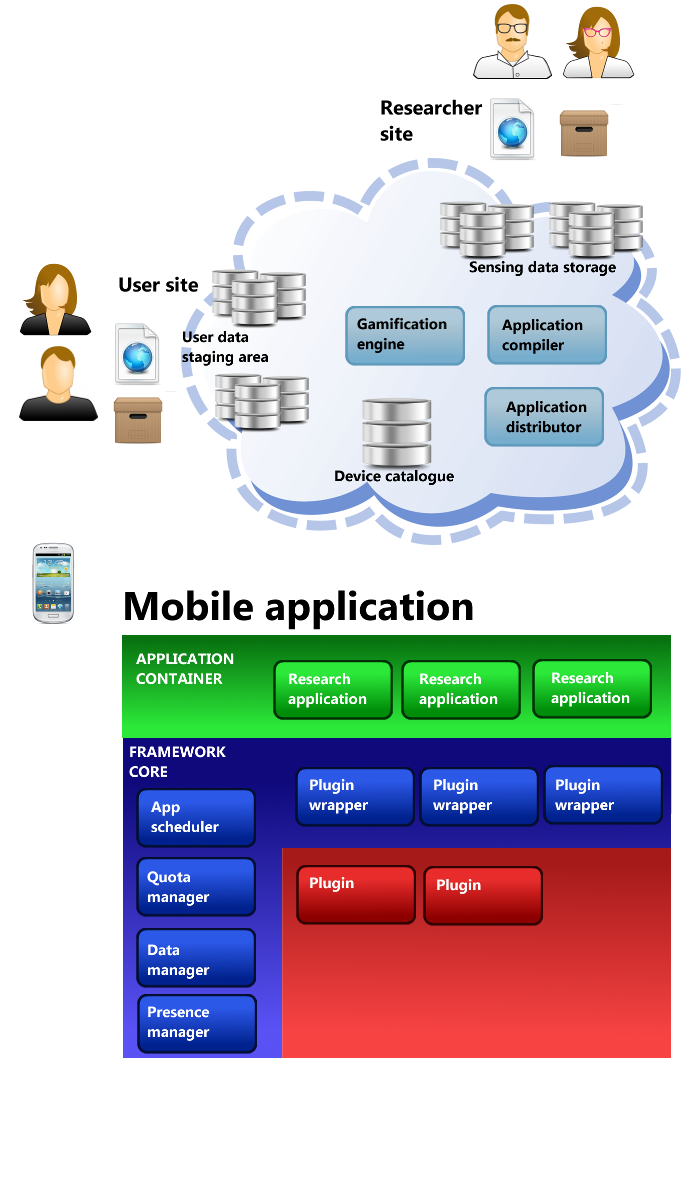
\includegraphics[width=\columnwidth]{structure.eps}
	\label{fig:structureImage}
\caption{DroidLab architecture}
\end{figure}
Figure 1 shows an overview of the DroidLab framework. In the center of DroidLab is the server. Different server components communicate with different client modules. The concept of DroidLab is that installations are configurable through plugins that the user can choose to install, and permissions that the user may or may not give to the client. This results in a heterogeneous device pool. On the other hand application developers arrive with different needs. The server's task is to match the needs with the resources, and handle the communication between the applications running on the client devices and the developers. The process is the following.\\
\indent Developers upload the source code of their application, along with a descriptor file containing the requirements towards the device and the installed DroidLab setup. The descriptor file is matched to the available device pool. If needs are met, the server compiles a downloadable binary, and pushes it to the device alongside with the granted permissions and resource quotas the application is allowed to consume. The packet is received by the App scheduler which in turn manages the lifecycle of the applications.\\
\indent Once an application is pushed to a device, the App scheduler takes care of its lifecycle. Applications can rely on timers and sensor events to trigger their operation. Applications can be written using a limited feature set of Java, building on top of a lightweight API, instead of using an own domain specific language. This way sensing tasks or protocols can exploit the full power of base Java classes to implement complex business logic. Sensor functionality is provided by the installed plugins. While plugins do the sensing tasks, plugins don't save sensor data. Sensor functions return with their results, which might than be processed or dropped by the application. Or compressed, aggregated with other sensors measurements and only then sent to the server. We decided to use this more flexible approach to limit bandwidth and storage space needs. Applications use the Data manager to persist information. The Data manager is responsible for the local storage of this information, and for the scheduling of the uploads.\\
\indent The fourth main component of the framework core is the Presence manager. In order for the server to work properly, a maintained device configuration is required. The Presence manager notifies the server about device configuration changes and  device state.
\begin{figure}[h]
\centering
	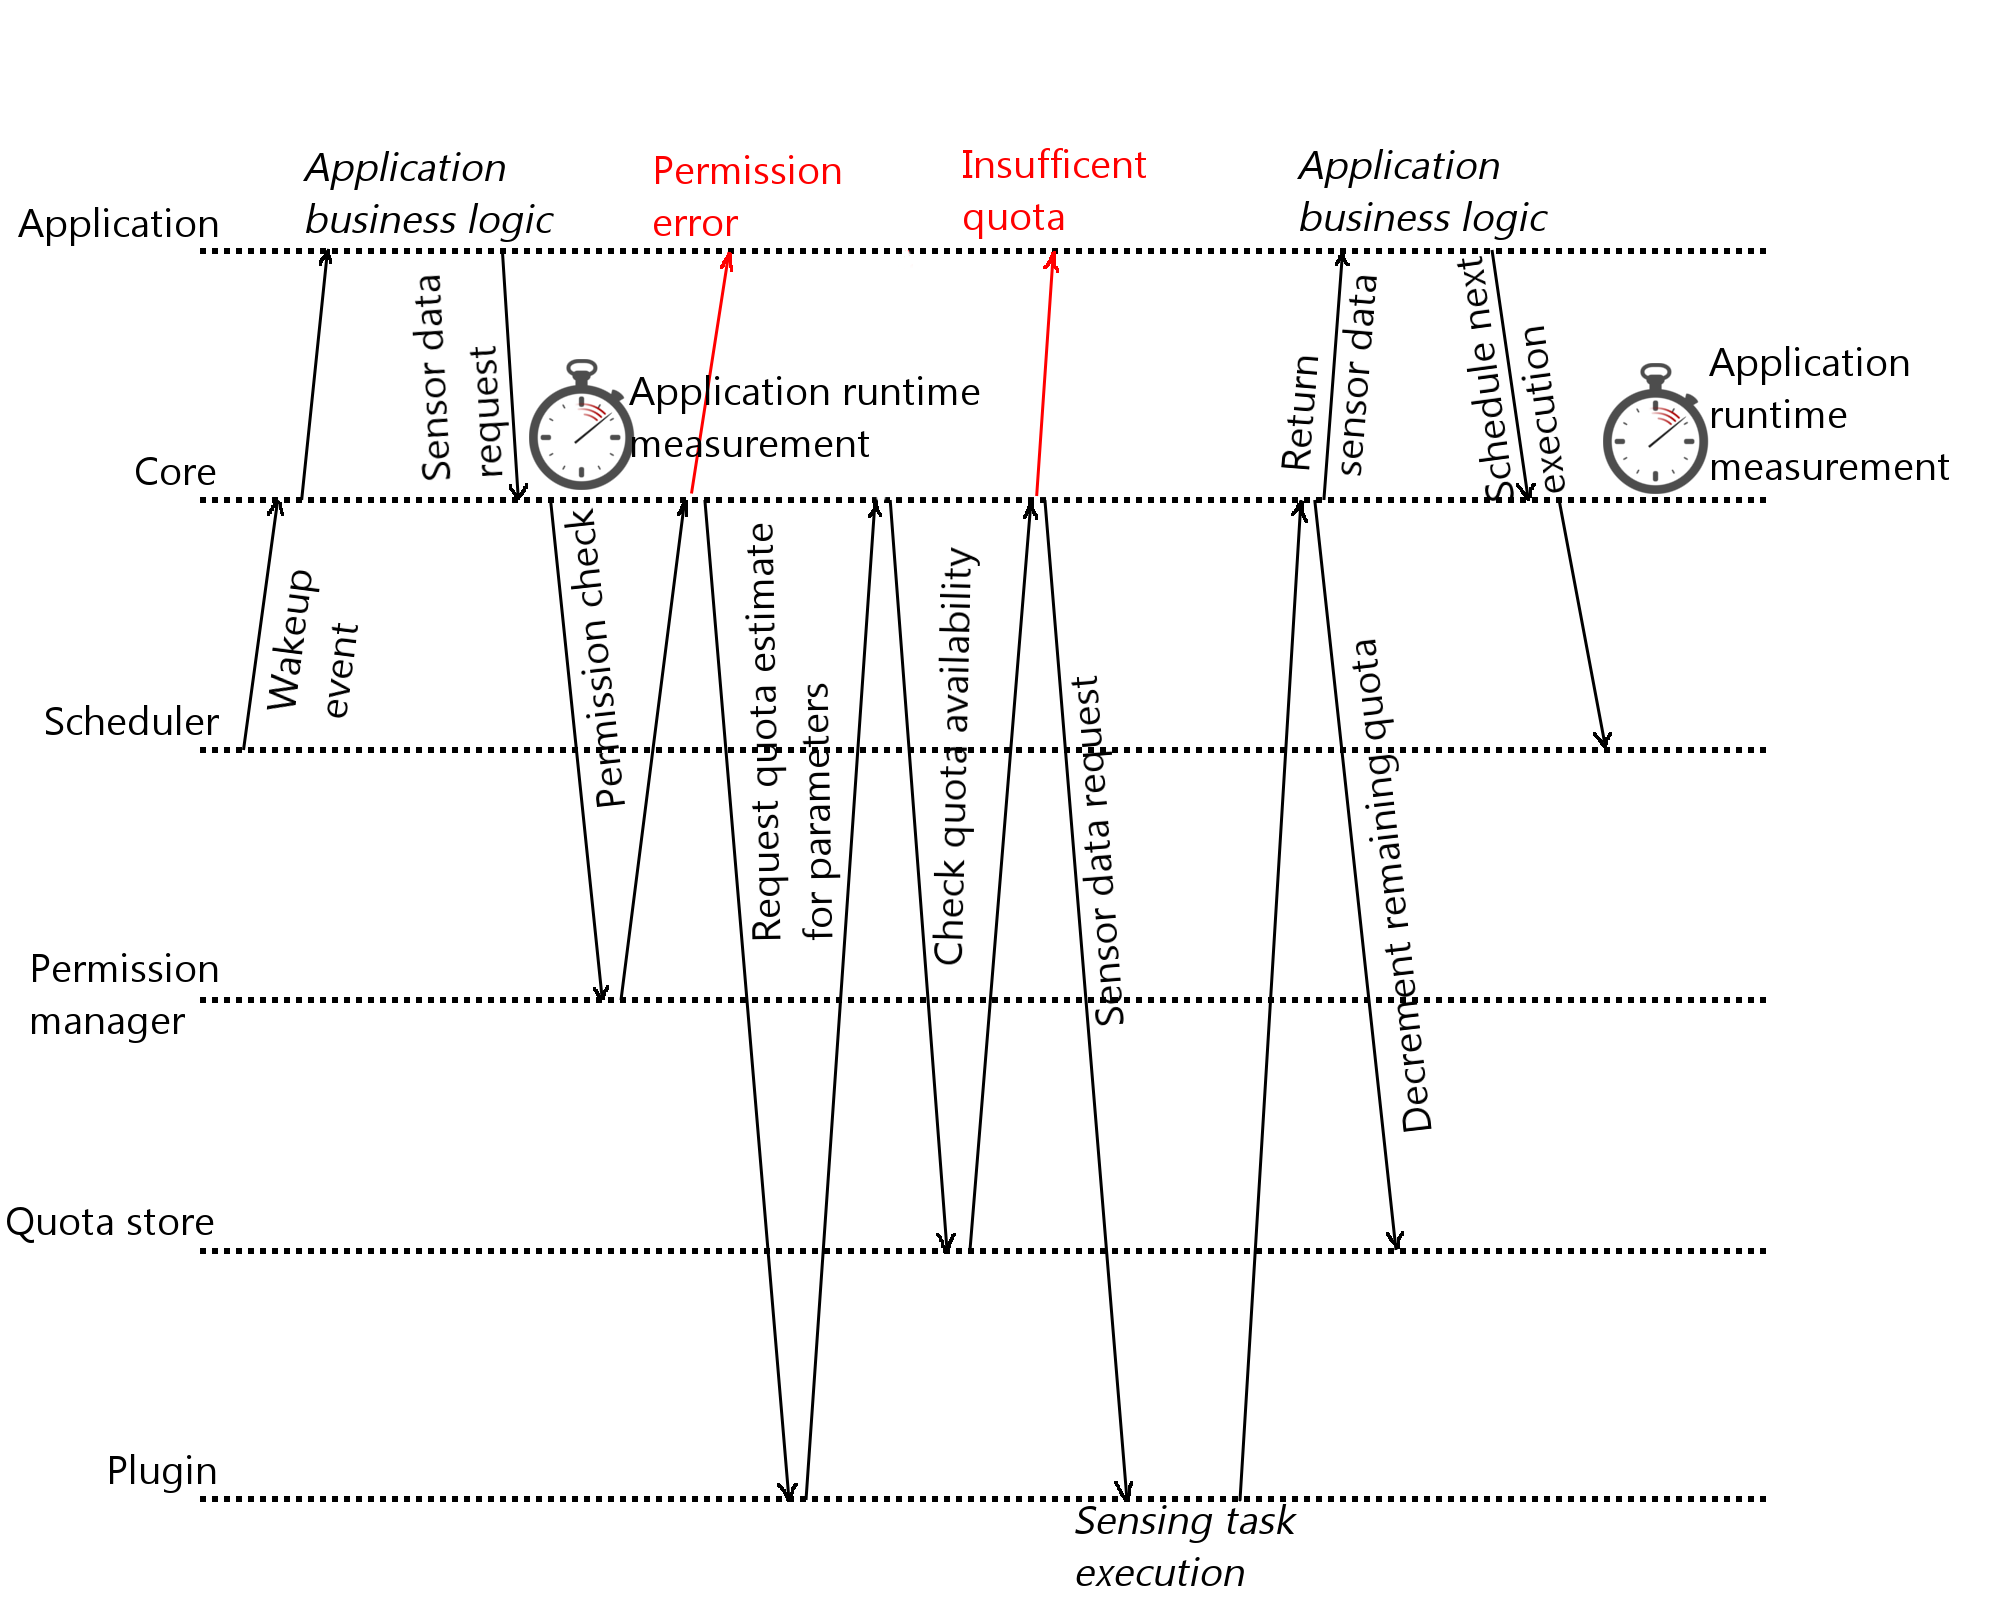
\includegraphics[width = \columnwidth]{communication.eps}
	\label{fig:communicationImage}
\caption{Sensing request sequence diagram}
\end{figure}
Applications run in a managed sandbox. Each delivered event and called method is monitored by the framework and authorized by the resource manager running on the device. Once the application's quota level is reached or the overall quota limit has expired, the framework denies the request. Figure 2 shows the control flow of a sensor access. It starts off by a trigger. Either the scheduler can notify the core about a timeout that has been scheduled, or a plugin fires an event based on sensor values. The Core finds the Applications that have to be launched. Applications get to run only for a very short time, and during this period they have to process the received event. In response they can initiate sensor readings, subscribe or unsubscribe from events, and set timers. If the application places a sensor request, a callback is registered and the framework handles the call asynchronously. First, permissions need to be checked. If the user authorized the call, the core asks for a quota estimate for the given parameter set from the plugins. If the application has enough credit for the call, the plugin method is called. When a plugin returns a result, the application's available credit is decremented, and the callback is called. This mechanism is both secure and flexible.\\
\indent Application terminates if one of the required quotas or predefined lifespans expires, the user explicitly removes it from the framework, a required permission is revoked, or a required plugin is uninstalled. Application is then removed from the device. Data generated by the application is cached until uploaded to the server.
\subsection{Challenges}
We faced several challenges during the design and development of the framework. Some of the challenges come from the goals we wanted to achieve, others were the result of the chosen architecture. We will briefly explain how DroidLab tackles them.
\subsubsection{Modularity}
The DroidLab framework, from an Android perspective, consists of a core application and plugin applications. Each plugin can be installed or removed as an Android application. Each plugin requires the permissions that are needed for its use. This enables the user to assemble a setup that he/she is comfortable with, and is suitable for the capabilities of the device. If the user doesn't want to share his/her location, then by omitting that plugin the framework will be limited on the OS level not to use the location services.\\
\indent The clear benefits of this modular approach come with some drawbacks. The DroidLab distributions will be fragmented, devices will have different plugin sets and even plugin versions. Users will also have the possibility to revoke permissions from the framework and limit the resource usage of plugins.
\subsubsection{Security}
DroidLab ensures that the user is protected from both outside attacks and malicious applications. We identified a number of high risk points in the architecture.\\
\indent We rely on Android Play Store's security measures to guarantee that neither the framework nor the plugin codes can be compromised. Both the framework and the plugins can be downloaded from the Play Store. This ensures that no third party application will be able to use the same package name on the device. The Android user management system ensures code integrity; thus, DroidLab isn't more fragile than any Android application.\\
\indent An attacker could compromise though the DroidLab client by pushing to the client an application that either has altered quotas and permissions, or contains code that was not checked and compiled on the DroidLab server. To prevent such an intrusion, every application and accompanying resource descriptor is signed by DroidLab's asymmetrical key. The application has the public key compiled inside itself. This signature is checked every time the application is loaded from local storage.\\
\indent Applications are written in Java, compiled by the server, and sent to the client. To make sure the client framework has full control over the application, only a limited set of the Java language can be used. Developers are limited to java.lang, java.util and java.math packages, excluding threading, Timer and class loading. Developers are allowed to use DroidLab's interfaces package, but cannot reference any class from the framework. Source code is checked for these imports and compiled without any external library. This ensures that applications cannot reach outside of the designated sandbox.\\
\indent Finally, DroidLab uses intents to communicate on the device between the different components. Android permissions are defined and enforced for these intents, limiting senders and receivers of the intent to the trusted components of the client (framework and plugins). It is up to the user to keep his device safe, any installed Android application has to be authorized, and permissions have to be granted manually.
\subsubsection{Privacy}
One of the main user concerns is privacy. A crowdsourcing framework can be successful only if the users can be certain that the data shared through the application doesn't violate their privacy. The required level of privacy varies from person to person, and DroidLab is designed to allow different levels of privacy.\\
\indent The common basis of privacy is device anonymity. Each device generates a unique identifier and every data is associated to that identifier. The identifier is independent of any other device or user identifier. That means that if a user reinstalls the application, the two installations will have different identifiers and cannot be associated. Nor can an attacker identify the user based solely on his DroidLab id. As the framework only handles the task of storing log lines generated by the applications, other privacy issues are taken in account on the plugin level. We design every plugin with user privacy in mind. Permissions defined by the plugins are designed in a way to accommodate different privacy needs. There is a trade-off between anonymity and sensory data value. Perturbing time and location information can conceal the user's identity form an attacker but compromises the sensing tasks precision. Similarly users might be identified from their social connection graph even if each node is anonymous. Such concerns will be addressed when designing the plugins' functionality.\\
\indent Prior to uploading, log files have to be stored on the external storage, as most current phones have limited internal storage available. These files can be read and altered by any application having permission to the SD card. To protect the sensitive information, we use a XOR symmetric key coding and sign the saved files. This guarantees integrity and privacy. Files will be uploaded through a secure channel either manually or automatically. In case of manual settings the user can review file contents before deciding to delete or upload them.\\
\indent Files uploaded to the server are stored in the user's private staging area. Users can access the information that will be shared by them. Three sharing options will be available to the user. Always share will grant developers access to the files immediately, speeding up the data processing. Share if not removed will grant developers access to the files after a given period, if the user didn't delete them Finally, the strictest option, share when permitted, keeps files private until the user doesn't give explicit permission to share the files with the developer. Files can be reviewed but not altered by the user.
\subsubsection{Seamlessness and resource management}
DroidLab will run on user equipment, tablets and phones that have to perform well, in a seamless manner their usual tasks, even when DroidLab is running resource-hungry sensing applications in the background. Moreover, these devices are mostly mobile, with limited or costly network access. Thus, all these aspects (limited battery, CPU and communication resources vs. seamless and efficient operation) have to be taken into account when designing the framework. \\
\indent Our preliminary experiments show that the framework in itself doesn't influence battery life. We created three passive monitoring applications: a battery meter, a CPU utilization capturer, and a running application capturer, all scheduled to run each second. Running these applications didn't increase the battery usage considerably, battery lifetime was not compromised.\\
\indent On the other hand, active sensing like the use of the gyroscope, the accelerometer, WiFi or Bluetooth discovery, or active bandwith measurements will naturally consume more battery. Plugins can be optimized to reduce power consumption. To prevent the framework from draining the battery, thresholds can be set by the user, when to disable battery intensive tasks, and when to stop the framework altogether.
Another battery intensive task is the periodic upload of the collected sensing data. As this usually is not a time sensitive task, the framework takes in consideration the user's network preference, and also his indications on the minimum battery level at which the framework should upload the gathered data.\\
\indent Current Android distributions don't support Android application level CPU limits and quotas, let alone thread-level CPU limits. So our options were limited in terms of processor usage management. As the DroidLab application source code is checked to prevent starting new threads, the lifecycle of the application is managed by the framework. We are measuring the runtime of each application method call and flagging applications that take too long to return. However, plugin methods initiated by the applications are asynchronous, hence we do not measure CPU load resulting from a plugin call directly. An estimation of the CPU usage of CPU intensive plugin method calls will be incorporated in the quotas defined by the plugins.\\
\indent Our application design guidelines suggest a timer or event based operation, with small tasks that aim to filter sensor data or change the state of the application. DroidLab was not intended to be a distributed mobile computation platform.
\subsubsection{Incentives}
Many crowdsourced applications provide value-added services to the users in return for their collaboration. Another approach is the introduction of micro-payment systems to incentivize users in participating. A micropayment system in an automated sensing scenario opens up however many issues. As opposed to easy to evaluate tasks, like answering a question or taking a picture at a given location, it is hard to put a price tag on a periodic or event based sensing task. A monetary reward would also attract cheaters. We believe thus that other extrinsic motivators should be used to increase public involvement. We propose a gamified approach. \\
\indent The framework in itself is just a delivery system for applications. Our goal is to be able to run more applications on more devices, and to be able to target specific user groups. This requires that users install more plugins,give more permissions and higher quotas. Moreover, they should provide detailed user profiles about themselves. \\
\indent On the other hand each application benefits from different user behaviors. A pothole detecting application needs car users. Drivers using roads that are not yet part of the database are more valuable than users taking the same path every day. For an application that maps open WiFi networks, people not switching on their WiFi connection, or devices used only at home are useless.\\
\indent We plan on implementing a gamified framework  that has both a unified and an application level reward system. The gamified system will be composed of points, leaderboards and badges. Points will be awarded for quotas that the applications spend. As developers have limited quota available, applications will be optimized to use fewer resources. So a quota spent by the application will bring value to the developer. Users will be also motivated to run more applications. The users to succeed in the game will have to make their setup desirable to the applications, meaning more plugin installations, permissions and higher quota limits. Leaderboars will be based on the points awarded to the users. With the increase of the user count, we will create different leaderboards for different time windows, and social leaderboards allowing users to compare themselves to their peers.\\
\indent Badges will help the application developers task and reward their users. Applications will have the possibility to define badges that will be part of the gamified system, will be present on the user profile, users will be able to share them on social network sites. Badges will be earned by meeting certain requirements or accomplishing meta-tasks. Specifications of the task that has to be accomplished to earn the badge can be secret or known to the user. In the latter case, the framework will present the user with the description of the task when the application is installed to give the user a chance to modify his behavior in order to gain the badge. The application will be responsible for checking whether the requirements have been fulfilled or not. The framework will also define badges, which will be part of the tutorial introducing the user to DroidLab. User tasks will guide the user through the settings, and give the user some insight about the system.
\subsubsection{Scaling}
As opposed to crowdsensing applications, DroidLab will not have bootstrapping issues. DroidLab doesn't provide a service that relies on sensing data, thus the first user will receive the same user experience as a user joining the system when it is already wide spread. In fact, early adopters will benefit from their history when it will come to leaderboards or badges: as badges are associated to applications, if an application is available for a limited time only, badges earned during that period will be more valuable. DroidLab's success won't depend on its startup speed.\\
\indent DroidLab's server requests needed for its operation scale linearly with the number of devices. Most of the server interactions consist of uploading or downloading files related to a single user or a single application. Most gamification related server requests will also require only a single user's information. Leaderboards will be cached and evaluated periodically. This makes the cloud an ideal platform for DroidLab. A more complex task is the distribution of applications among devices. Finding an optimal solution is a hard problem. We will thus use sub-optimal algorithms to find acceptable associations. This will result in sub-optimal device quota usage, but will conserve server resources and make the system more resilent to high user count.
\section{Conclusions}
\label{sec:conclusion_and_future_work}
With the radical increase in the number of Android smart phones, the number of application developers has also steadily grown. Lots of useful and useless Android applications emerge constantly, some of them become very popular, almost independently of their usefulness, while others don't. Writing and testing an application that runs in parallel on a number of mobile devices and builds on the cooperation of several users is usually not an easy task on its own. In addition, the right incentives should be found to convince a critical mass of users to install and run the application to be tested, which is sometimes even harder than writing the application itself. \\
\indent DroidLab is being developed to handle exactly these problems. Application developers can upload their code on a large-scale Android testbed, run their experiments, test their algorithms, and gather the results in a straightforward way. On the other hand, users who are willing to install the DroidLab framework on their personal smartphones will have the possibility to control and monitor the resources consumed in the background, their interaction will not be needed, but their security and privacy will be ensured, thanks to the sandboxed approach used in the implementation of the framework.  Mobile crowd-sensing applications are the perfect targets of DroidLab, as we analyzed throughout this paper. However, other application scenarios can also be envisaged. Being developed as part of the FITTING European research project, DroidLab intends to be part of a federated global test environment, next to infrastructures such as PlanetLab and SensLab, providing a leap ahead in the development of applications and services running in the heterogeneous environments of the Future Internet.       
\bibliographystyle{plain}
\bibliography{droidlab,droidlab_manual}
\end{document}
%%% Local Variables: 
%%% mode: latex
%%% TeX-master: t
%%% End: